\section{Dynamic model}\label{sec:backstepping:dynamic_model}

We consider the robot made by a sequence of $n_{\mathrm{S}}$ segments. Each segment is described with $n_{\mathrm{D}}$ configuration variables by using one of the many modeling techniques are being developed in the state of the art~\cite{faure2012sofa, grazioso2018geometrically, sadati2019TMTDyn, boyer2020dynamics}.
%
We denote with $n_{\mathrm{q}} = n_{\mathrm{S}} n_{\mathrm{D}}$ the total number of configuration variables, which also represents the approximated DoFs of the soft arm.
%
Although we show planar kinematic relations for the \gls{PCC}-case in Figure~\ref{fig:backstepping:pcc_case_overview} as an example, the dynamic model derived in this section is agnostic to the chosen kinematic approximation.
%

All of kinematic modeling techniques produce multi\--body dynamics of the unactuated soft robot as follows~\cite{della2023model}
%
\begin{equation}
	B(q)\ddot{q} + C(q,\dot{q}) \dot{q} + G(q) + K(q) + D(q, \dot{q}) = 0,
\end{equation}
%
where $q \in \mathbb{R}^{n_{\mathrm{q}}}$ describes the configuration of the robot in generalized coordinates, $B(q) \in \mathbb{R}^{n_{\mathrm{q}} \times n_{\mathrm{q}}}$ the inertial matrix, $C(q,\dot{q}) \in \mathbb{R}^{n_{\mathrm{q}} \times n_{\mathrm{q}}}$ contains the Coriolis and Centrifugal forces and $G(q) \in \mathbb{R}^{n_{\mathrm{q}}}$ compensates for the gravitational effects. The elastic (restoring) forces are captured in the matrix $K \in \mathbb{R}^{n_{\mathrm{q}}}$ and the natural damping is represented by $D(q,\dot{q}) \in \mathbb{R}^{n_{\mathrm{q}}}$.

%
Each segment is actuated through a set of $n_{\mathrm{C}}$ dedicated chambers.
%
Adapting the pressure in a chamber will lead to to a different chamber volume and ultimately resulting in a changed configuration of the segment.
%
Each chamber is connected to a dedicated piston as shown in Figure~\ref{fig:backstepping:pcc_case_overview}. If more than one chamber is connected to a same piston, it can be considered to be the same chamber for the sake of this work.
%
These hypotheses are not paramount, but they are instrumental to maintain the notation easier.
%
Accordingly, the total number of pistons is described with $n_{\mu_\mathrm{p}} = n_{\mathrm{S}} n_{\mathrm{C}}$.
%
Please note that if $n_\mathrm{C} = n_\mathrm{D}$, the model of the soft robot is fully-actuated, if $n_\mathrm{C} > n_\mathrm{D}$ it is over-actuated, and with $n_\mathrm{C} < n_\mathrm{D}$ under-actuated respectively.
%
The dynamics of the piston when not interacting with the fluid can be easily written as being
%
\begin{equation}
M_\mathrm{p} \ddot{\mu}_\mathrm{p} + D_\mathrm{p} \dot{\mu}_\mathrm{p} + G_{\mathrm{P}}^{\mu_p} = f_\mathrm{p},
\end{equation}
%
where $\mu_\mathrm{p} \in \mathbb{R}^{n_{\mu_\mathrm{p}}}$ denoting the displacement of every piston from the zero-volume configuration, $M_\mathrm{p} \in \mathbb{R}^{n_{\mu_\mathrm{p}} \times n_{\mu_\mathrm{p}}}$ the mass matrix of the piston system, $G_{\mathrm{P}}^{\mu_p} \in \mathbb{R}^{n_{\mu_\mathrm{p}}}$ describing the conservative force caused by the compressed fluid acting on the pistons, and $D_\mathrm{p} \in \mathbb{R}^{n_{\mu_\mathrm{p}} \times n_{\mu_\mathrm{p}}}$ the damping matrix of the piston system. 
As the piston system is fixed to the ground and connected via tubing to the robot chambers, note that the gravity force here is constant, so w.l.o.g. we consider it to be zero (or alternative as being compensated by a constant off\--set in $f_\mathrm{p}$).

\begin{figure}[ht]
  \centering
  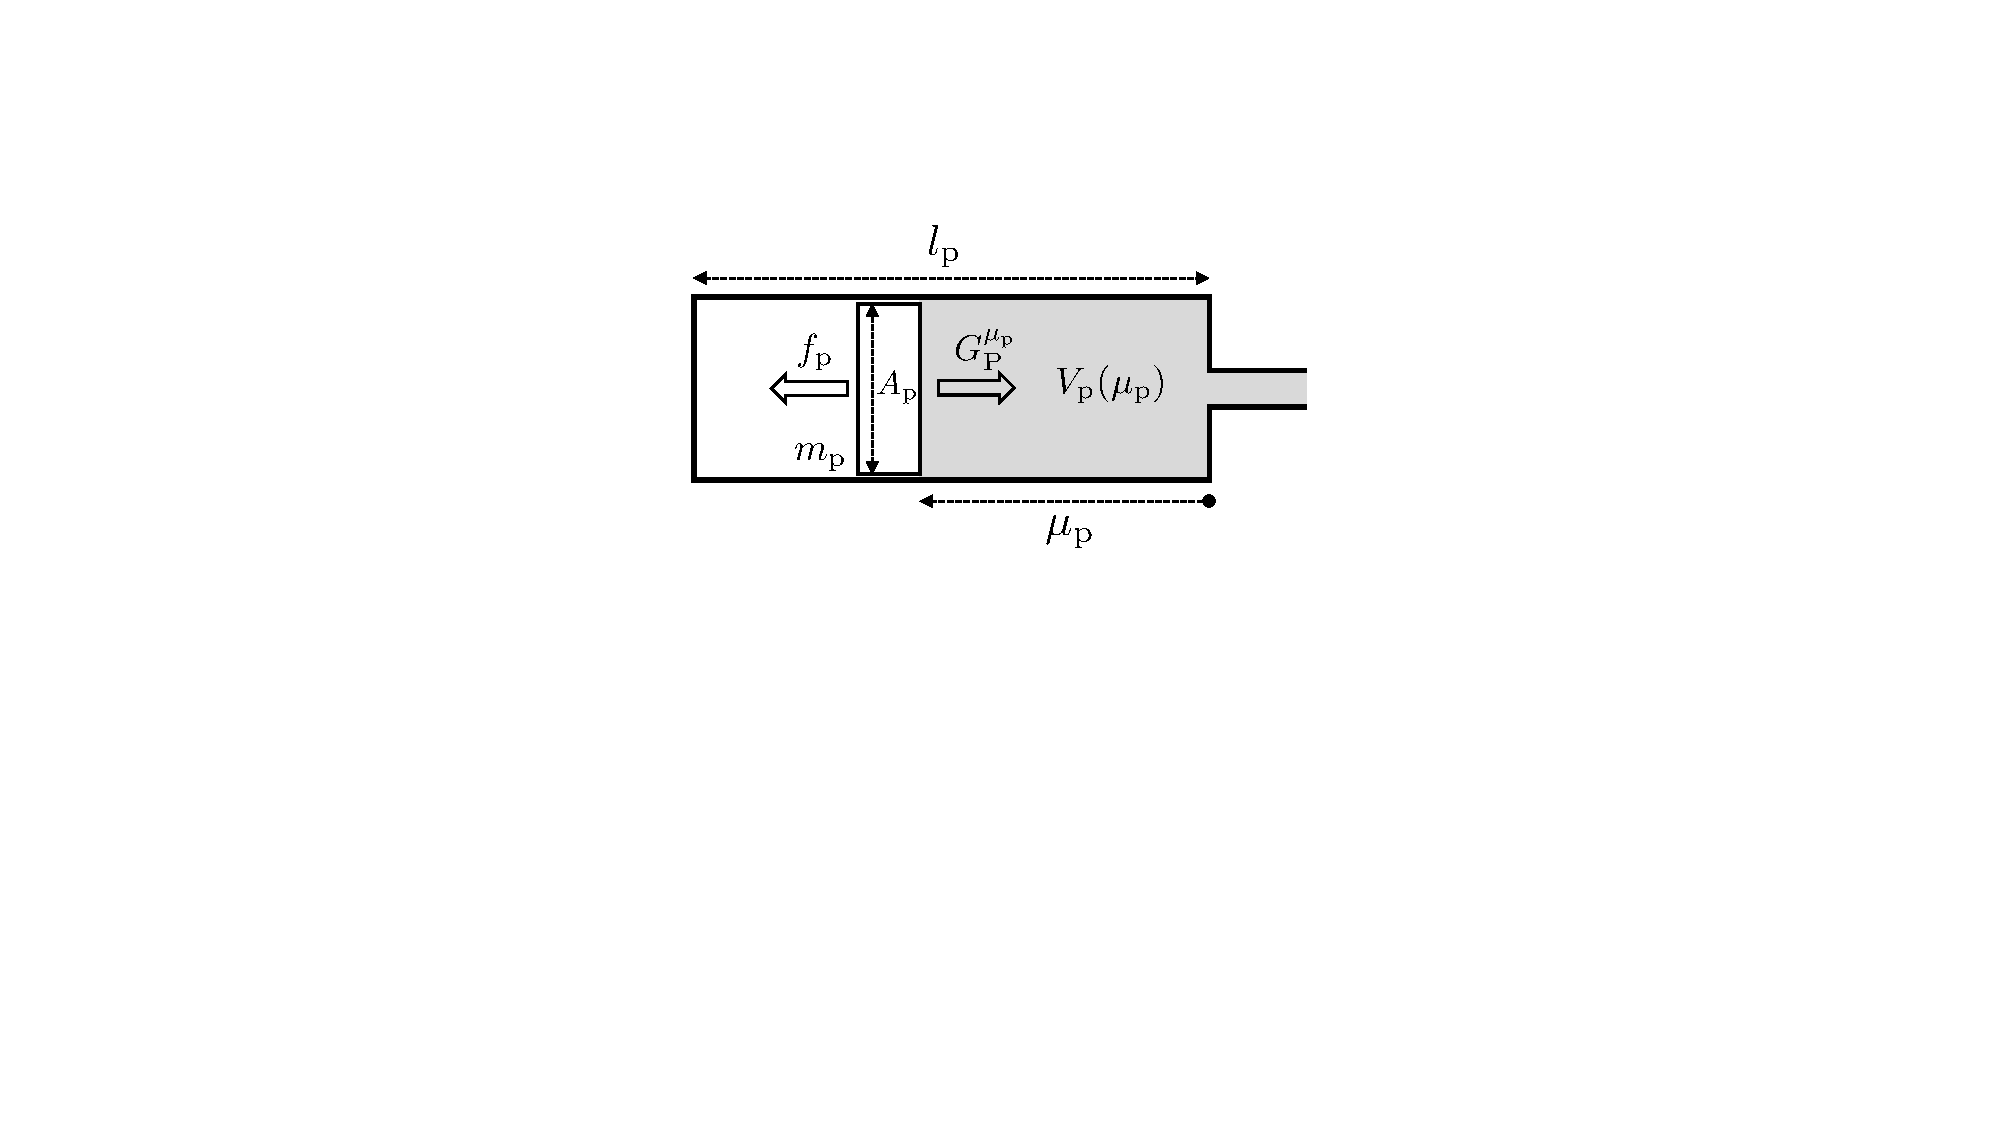
\includegraphics[width=0.5\columnwidth]{backstepping/figures/backstepping_graphics_fluidic_drive_cylinder_v4.pdf}
  \caption{Fluidic drive cylinder parameters for a piston of mass $m_\mathrm{p}$, length $l_\mathrm{p}$ and cross-sectional area $A_\mathrm{p}$: $f_\mathrm{p}$ describes the actuation force while $G_\mathrm{P}^{\mu_\mathrm{p}}$ is the conservative force applied by the compressed fluid on the cylinder. $\mu_\mathrm{p}$ represents the actuators' state variable. These pneumatic pistons could be for example actuated by current-controlled DC motors or linear electric actuators~\cite{marchese2014design}.}\label{fig:backstepping:fluidic_drive_cylinder}
\end{figure}

\begin{figure}[ht]
  \centering
  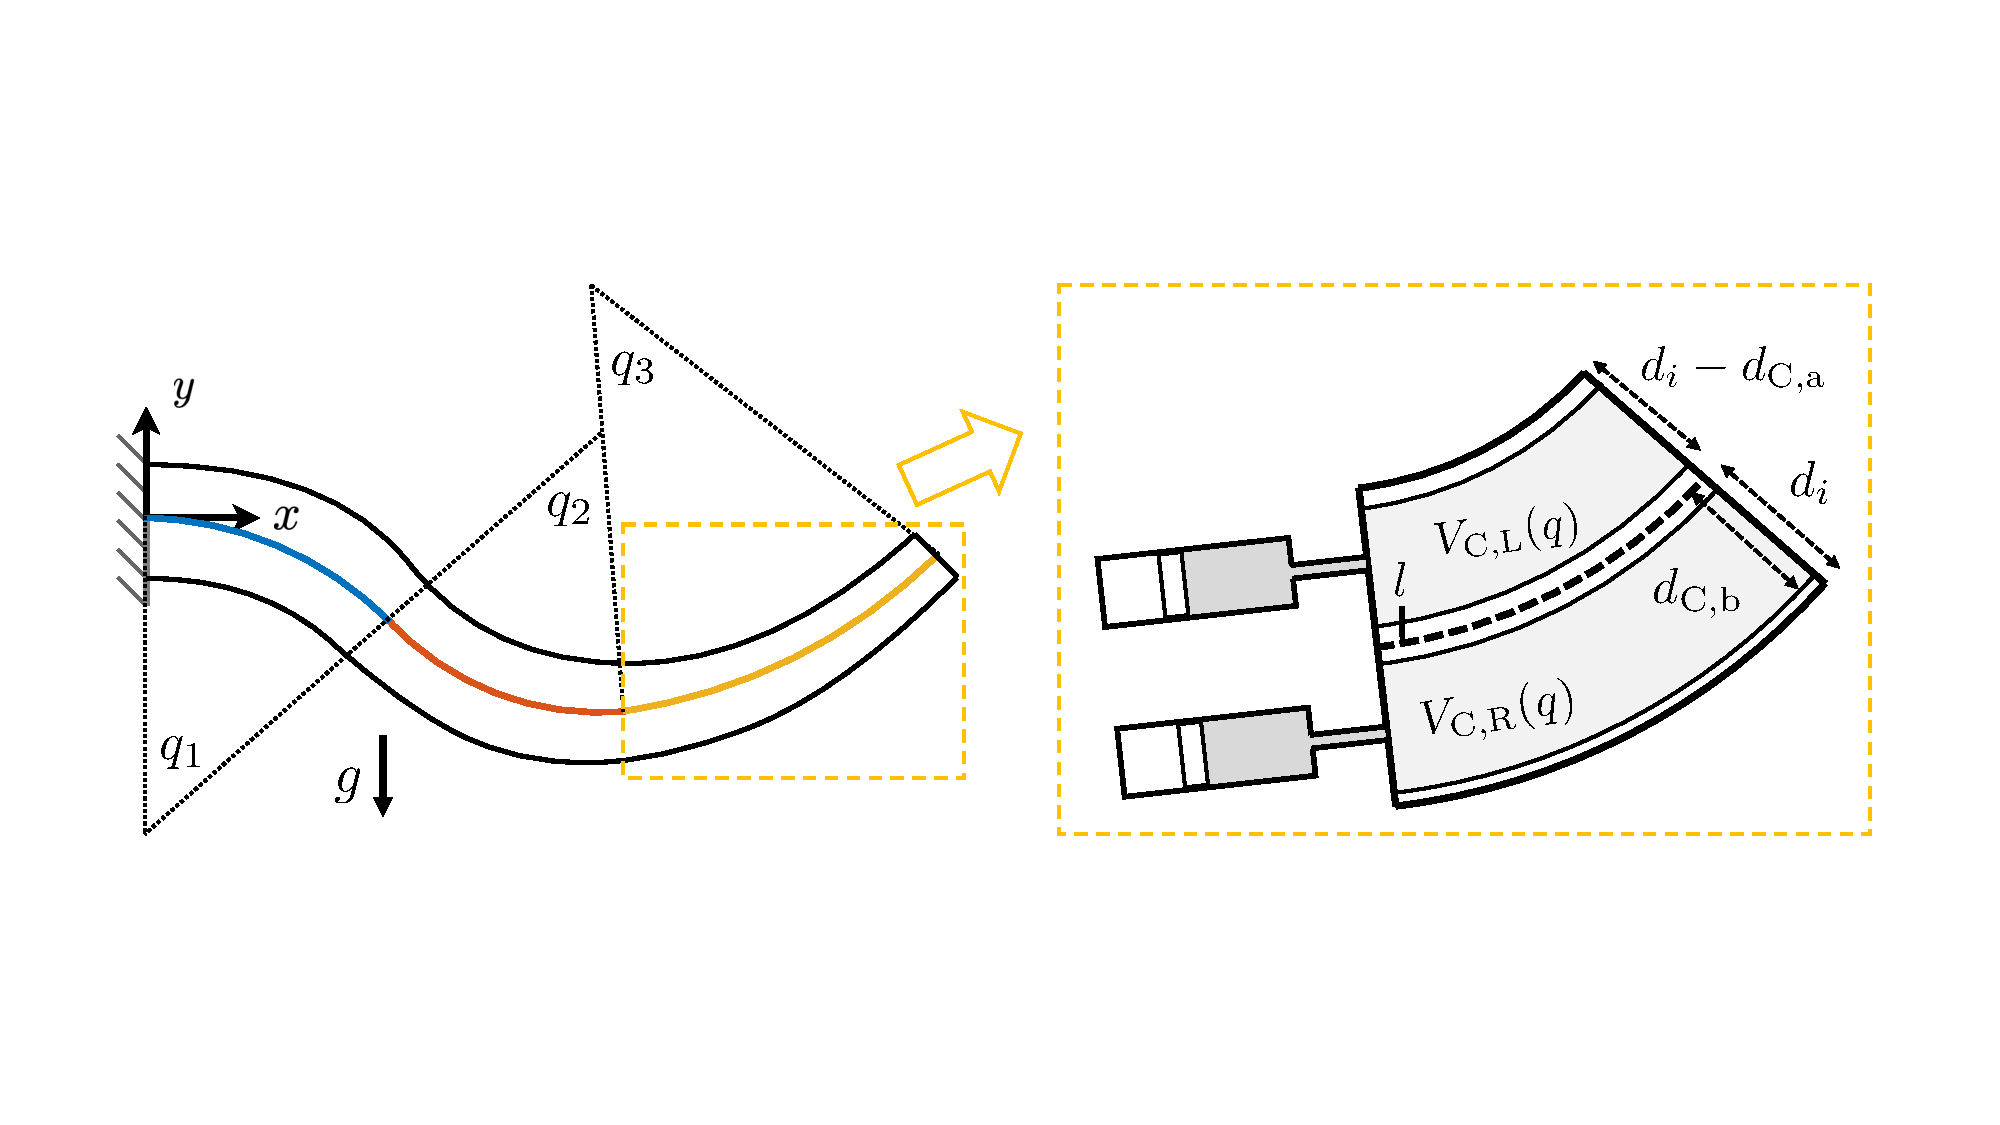
\includegraphics[width=0.9\columnwidth]{backstepping/figures/backstepping_graphics_pcc_case_overview_v4_cropped.pdf}
  \caption{Shape regulation under \gls{PCC} approximation - \textbf{Left:} A planar soft robot consisting of three segments each modelled to have constant curvature \textbf{Right:} Model parameters for fluidic volume in soft segment chambers. Each chamber is actuated independently by a fluidic drive cylinder connected through tubing.}\label{fig:backstepping:pcc_case_overview}
\end{figure}


In first approximation, we model the compressible fluid (typically air) as an ideal gas. Furthermore, we consider the process to be isothermal and that no exchange of fluid with the external world is happening. We neglect the volume of fluid in any tubes connecting the pistons with the chambers.
%
The overall volume of the fluid can be evaluated as %the sum of the chamber volume $V_{\mathrm{q},i}(q)$
%
%\begin{equation}
%	V_i(q_i,l_{c(i)}) = \sum_{j \in c(i)} V_{\mathrm{q},j}(q_i) + A_{c(i)}^{\mathrm{T}}  l_{c(i)}, 
%\end{equation}
%%
%where $c:\mathbb{N} \rightarrow \mathbb{N}^{n_{\mathrm{C}}}$ is the function returning the indexes of chambers actuating the $i\--$th segment.
\begin{equation}
V(q,\mu_\mathrm{p}) = V_{\mathrm{C}}(q) + V_{\mathrm{p}}(\mu_{\mathrm{p}}) = V_{\mathrm{C}}(q) + A_{\mathrm{p}} \mu_{\mathrm{p}}, 
\end{equation}
%
where $V(q,\mu_\mathrm{p}) \in \mathbb{R}^{n_{\mu_\mathrm{p}}}$ describes the total volume of fluid stored in the system, $V_{\mathrm{C}}(q) \in \mathbb{R}^{n_{\mu_\mathrm{p}}}$ the volume of fluid in each chamber and $V_{\mathrm{p}}(q) \in \mathbb{R}^{n_{\mathrm{S}} n_{\mathrm{p}}}$ the volume in the piston with $A_{\mathrm{p}} \in \mathbb{R}^{n_{\mu_\mathrm{p}}}$ the cross-sectional area of every piston.
%
% The function $V_{\mathrm{C}}(q)$ can be either analytically derived or learned off\--line from data. 
% move the following potentially to future work
% A possibility that we do not investigate here for the sake of space is to parametrize $V_{\mathrm{C}}(q)$  w.r.t. a set of unknown quantities $\pi$, and then learn $\pi$ on\--line through adaptive control.
%
We will present an example of analytical derivation of $V_{\mathrm{C}}(q)$ in Section~\ref{sub:backstepping:pcc_model}.
For now we consider it known.

The total energy stored in the system due to fluid compression is
%
\begin{equation}
\begin{split}
	\mathcal{U}_\mathrm{fluid}(q,\mu_\mathrm{p}) =& \: \sum_{j = 1}^{n_{\mu_\mathrm{p}}} \int_{V_{j,0}}^{V_j(q_i,\mu_{\mathrm{p},j})} -\left ( p_j(\nu) - p_\mathrm{atm} \right ) \mathrm{d} \nu\\
	% = \sum_{j = 1}^{n_{\mu_\mathrm{p}}} \alpha_{\mathrm{air},j} \int_{V_{j,0}}^{V_j(q,\mu_\mathrm{p})} -\left ( \frac{1}{\nu} - \frac{1}{V_{j,0}} \right ) \mathrm{d} \nu\\
	=&\: \sum_{j=1}^{n_{\mu_\mathrm{p}}} - \alpha_{\mathrm{air},j} \left ( \ln  \frac{V_j(q_i, \mu_{\mathrm{p},j})}{V_{j,0}} - \frac{V_j(q_i, \mu_{\mathrm{p},j})}{V_{j,0}} + 1 \right ),
\end{split}
\end{equation}
%
where $V_j(q_i, \mu_{\mathrm{p},j}) = \frac{\alpha_{\mathrm{air},j}}{p_j(q_i, \mu_{\mathrm{p},j})}$ represents the total fluidic volume in the system of chamber and piston $j$ in segment $i$. We assume that this fluid system is filled with air at atmospheric pressure $p_\mathrm{atm}$ with an initial volume of $V_{j,0} = V_j(0, l_\mathrm{p})$ (e.g. straight robot configuration and with fully extended pistons). 
This lets us find an expression for $\alpha_{\mathrm{air}}$:
\begin{equation}
    \alpha_{\mathrm{air},j} = n_j R T = p_\mathrm{atm} V_{j,0} = p_{j}(q,\mu_\mathrm{p}) V_{j}(q,\mu_\mathrm{p}).
\end{equation}
%
% More complex pressure\--volume relationships involving not constant $n_j$ will be the topic of future investigations.

The force exerted on the $i$th segment of the robot by the fluid is 
%
%\begin{equation}
%		G_{\mathrm{P},j}^{\mathrm{q}}(q,l) = \partial_{q_j} E =  \sum_{i \in c(j)} \alpha_i \frac{\partial_{q_j}V_{\mathrm{q},i}}{V_{\mathrm{q},i}(q) + A_i l_i}, 
%\end{equation}
\begin{equation}\label{eq:backstepping:GPq}
\begin{split}
    G_{\mathrm{P},i}^{\mathrm{q}}(q_i,\mu_{\mathrm{p},j}) &= \partial_{q_i} \mathcal{U}_\mathrm{fluid}(q,\mu_\mathrm{p}) = -\partial_{q_i} V_{C,j} \left ( p_{j}(q_i, \mu_{\mathrm{p},j}) - p_\mathrm{atm} \right ), 
\end{split}
\end{equation}
Similarly, the force applied on $j$th piston by the fluid is
%
\begin{equation}\label{eq:backstepping:GPmu}
\begin{split}
    G_{\mathrm{P},j}^{\mu_\mathrm{p}}(q_i,\mu_{\mathrm{p},j}) &= \partial_{\mu_{\mathrm{p},j}} \mathcal{U}_\mathrm{fluid}(q,\mu_\mathrm{p}) = - A_{\mathrm{p},j} \left ( p_{j}(q_i, \mu_{\mathrm{p},j}) - p_\mathrm{atm} \right ), 
\end{split}
\end{equation}
%
The overall dynamic model is
%
\begin{equation}\label{eq:backstepping:complete_dyn} %
\begin{split}
	B(q)\ddot{q} \!+\! C(q,\dot{q})\dot{q} \!+\! G(q) \!+\! K(q) \!+\! D(q,\dot{q}) \!+\! G_{\mathrm{P}}^{\mathrm{q}}(q,\mu_\mathrm{p}) &= 0, \\
	M_\mathrm{p} \ddot{\mu}_\mathrm{p} + D_\mathrm{p} \dot{\mu}_\mathrm{p} + G_{\mathrm{P}}^{\mu_\mathrm{p}}(q,\mu_\mathrm{p}) &= f_\mathrm{p}, \; 
\end{split}
\end{equation}
which is always underactuated.
%
Note that this structure is similar to the one of classic flexible joint robots under Spong's approximation \cite{della2021flexible} due to the fact that the fluidic drive cylinders are fixed to the ground. Two of the major differences making the control problem harder are that that $n_{\mu_\mathrm{p}} \neq n_{\mathrm{q}}$, and that $G_{\mathrm{P}}^{\mathrm{q}}$ and $G_{\mathrm{P}}^{\mu_\mathrm{p}}$ are not linear.
The latter renders the feedback coupling of the outer on the inner subsystems non-affine.
%
In the rest of the paper, we will use the following definitions to simplify the notation
%
\begin{small}
\begin{equation}\label{eq:backstepping:gf}
\begin{split}
	f(q,\dot{q}) &= - B^{-1}(q)\left(C(q,\dot{q})\dot{q} + G(q) + K(q) + D(q, \dot{q}) \right), \\
	g(q,\mu_\mathrm{p}) &= - B^{-1}(q) \left ( G_{\mathrm{P}}^{\mathrm{q}}(q,\mu_\mathrm{p}) \right ).
\end{split}
\end{equation}
\end{small}